\documentclass[12pt, A4Paper]{article}
\usepackage[utf8]{inputenc}
\usepackage{graphicx}

\title{Smart Garage}
\author{Fabiha Tasneem }
\date{August 2022}

\begin{document}

\begin{titlepage}
   \begin{center}

       \LARGE{\textbf{Computer Security Project Report}}

       \vspace{1cm}
       \Large{\textbf{CSE 406}}\\
       \vspace{0.5cm}
       \large{\textbf {Tool: Snort}}
       
        \vspace{2cm}
    \textbf{Supervisor:}\\
       Sayem Hasan\\
       Adjunt Lecturer\\
       CSE, BUET\\
       
       
      \vspace{3cm}
    \textbf{Presented By:}\\
       Farhan Tanvir - 1805073\\
       Kowsar Mahmud Pappu - 1805075
            
       \vspace{2cm}
        Level-4 Term-1\\
        Department of CSE\\
       Bangladesh University of Engineering \& Technology\\
       13 September, 2023\\
            
   \end{center}
\end{titlepage}

\section{Tool Overview}
Snort is an open source network intrusion detection and prevention system (IDS/IPS) tool. It is widely used for real time traffic analysis and packet logging on IP networks. Here is an overview of Snort's key features and functionalities:

\begin{enumerate}
    \item \textbf{Intrusion Detection:} Snort can detect and alert on various types of network-based attacks, including
    \begin{itemize}
        \item Unauthorized accesses
        \item DoS attacks
        \item Malware infections
    \end{itemize}

    \item \textbf{Rule-Based Detection:} Snort uses a rule-based detection engine to analyze network traffic and compare it against a set of predefined rules. These rules can be customized to match specific attack signatures or patterns

    \item \textbf{Protocol Analysis:} Snort supports the analysis of multiple network protocols, including TCP, UDP, ICMP, and more. It can inspect packet headers and payloads to identify anomalies or malicious activities

    \item \textbf{Traffic Analysis and Statistics:} Snort provides detailed statistics and reports on network traffic, including the number of alerts triggered, traffic volume, and attack trends. This information can be used for network monitoring and security analysis
\end{enumerate}
\vspace{0.4cm}

\section{Source Code Overview}
The central component of Snort setup resides in its configuration file, typically located at \textbf{\textit{/etc/snort/snort.conf}}. Within this configuration file, crucial details regarding both the internal and external network settings utilized by the tool are specified. Additionally, it serves as the repository for defining ports and protocols. Furthermore, provisions for implementing whitelists and blacklists are embedded in this configuration file. \textbf{It comes equipped with a set of default rules, while users have the flexibility to craft their own custom rules in \textit{/etc/snort/rules/local.rules}}. The rules directory contains an array of rule definitions distributed across multiple files and the local.rules file (initially empty) serves as a canvas for users to append their personalized rule set as per their requirement.
\vspace{0.4cm}

\section{Feature Description}
Snort can be configured to operate in three different modes.

\begin{enumerate}
    \item \textbf{Sniffer Mode:}
    \begin{itemize}
        \item In Sniffer mode, Snort functions as a passive network sniffer or packet logger
        \item It generates alerts and logs based on predefined rules but does not actively block or prevent network traffic
        \item Sniffer mode is typically used for network monitoring, packet capture, and analysis to understand network activity and identify potential security threats
    \end{itemize}

    \item \textbf{Logger Mode:}
    \begin{itemize}
        \item In Logger Mode, Snort captures and logs network packets but does not generate alerts or take immediate action
        \item It is useful for network administrators who want to record network traffic for later analysis or auditing without immediate intrusion detection or prevention
        \item While it does not actively prevent attacks, it provides valuable information for post-incident analysis
    \end{itemize}

    \item \textbf{Network Intrusion Detection System (NIDS) Mode:}
    \begin{itemize}
        \item In this mode, Snort actively monitors network traffic, analyzes packets in real-time, and generates alerts for suspicious or malicious activity based on predefined rules
        \item Unlike the previous modes, NIDS Mode can take action to block or drop malicious traffic, making it an intrusion prevention system (IPS)
    \end{itemize}
\end{enumerate}
\vspace{2.5cm}

\section{Feature Documentation}
\begin{enumerate}
    \item \textbf{\large{Packet Sniffing (Sniffer Mode):}}
    \begin{itemize}
        \item \textbf{sudo nano /etc/snort/snort.conf}\\ 
    - This command opens snort.conf in the nano editor
        \begin{figure}[h]
            \centering
            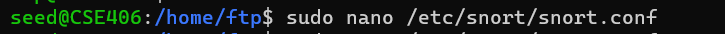
\includegraphics{images/sudo_nano_conf}
        \end{figure}
        
        \item Check if \textbf{ipvar HOME\_NET} is set to \textbf{your subnet} (e.g. 10.0.0.0/24)
        \begin{figure}[h]
            \centering
            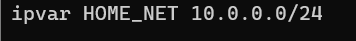
\includegraphics{images/HOME_NET}
        \end{figure}

        \item Comment all the included custom rules like \textbf{include \$RULE\_PATH/$<$filename$>$.rules} by appending \# at the front so that we can write our own rules and test them
        \begin{figure}[h]
            \centering
            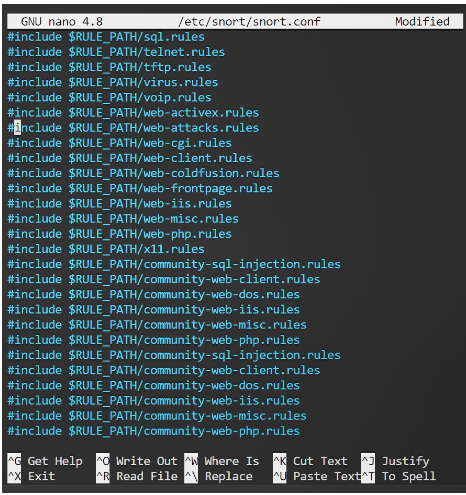
\includegraphics[width=0.25\textwidth]{images/comment_rules.PNG}
        \end{figure}

        \item Control + O → Enter → Save changes in nano\\
        Control + X → Exit nano

        \item \textbf{sudo snort -T -i eth0 -c /etc/snort/snort.conf}\\ 
    - This command tests if everything is alright in the configuration file
        \begin{figure}[h]
            \centering
            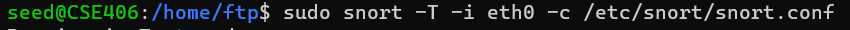
\includegraphics{images/test_conf}
        \end{figure}

        \item \textbf{sudo nano /etc/snort/rules/local.rules}\\ 
    - This command opens the \textbf{local.rules} file in nano
        \begin{figure}[h]
            \centering
            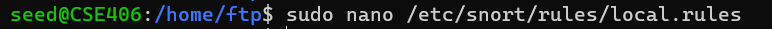
\includegraphics{images/sudo_nano_rules}
        \end{figure}

        \item \textbf{alert icmp any any $->$ 10.0.0.4 any (msg:”ICMP Ping Detected”; sid:100001; rev:1;)}\\ 
        - Write this rule in the last line of the local.rules file. This is a rule that detects any ICMP packet, that is, ping towards the home network from anywhere and generates an alert\\

        \textbf{alert tcp any any $->$ 10.0.0.4 21 (msg:"FTP Connection Attempt"; sid:100003; rev:1;)}\\ 
        - This rule detects any FTP connection attempt
        \begin{figure}[h]
            \centering
            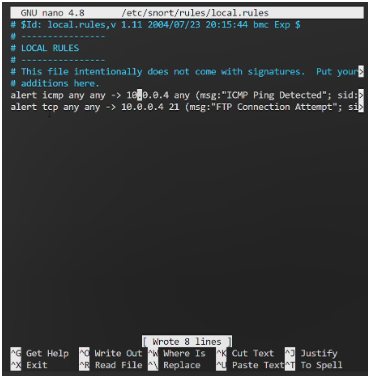
\includegraphics[width=0.4\textwidth]{images/add_rules}
        \end{figure}

        \item Save and Exit Nano

        \item \textbf{sudo snort -q -i eth0 -A console -c /etc/snort/snort.conf}\\ 
    - This command starts Snort in quiet mode, sniffs packets from the eth0 interface and prints an alert on the console
        \begin{figure}[h]
            \centering
            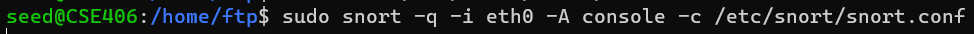
\includegraphics[width=0.95\textwidth]{images/start_snort}
        \end{figure}
    \end{itemize}
    
    \item \textbf{\large{Packet Logging (Logger Mode):}}
    \begin{itemize}
        \item \textbf{sudo nano /etc/snort/rules/local.rules}\\ 
    - This command opens the \textbf{local rules} file in nano
        \begin{figure}[h]
            \centering
            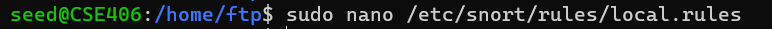
\includegraphics{images/sudo_nano_rules}
        \end{figure}

        \item \textbf{alert tcp any any $->$ 10.0.0.4 21 (msg:"FTP Connection Attempt"; sid:100003; rev:1;)}\\ 
        - Write this rule in the last line of the local.rules file. This rule detects any FTP connection attempt
        \begin{figure}[h]
            \centering
            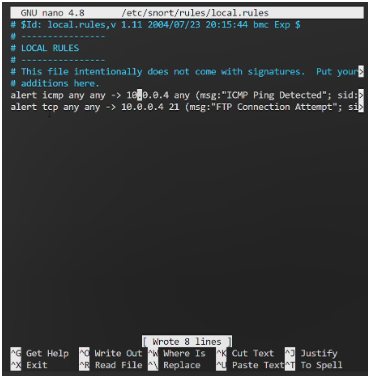
\includegraphics[width=0.4\textwidth]{images/add_rules}
        \end{figure}

        \item \textbf{sudo snort -q -l /var/log/snort -i eth0 -A console -c /etc/snort/snort.conf}\\
        - This command starts Snort in quiet mode, sniffs packets from the eth0 interface, logs everything about it in the \textbf{/var/log/snort} directory and prints an alert on the console
        \begin{figure}[h]
            \centering
            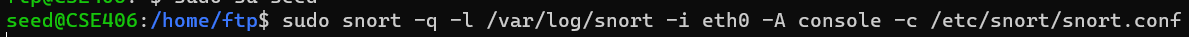
\includegraphics[width=0.95\textwidth]{images/start_snort_log}
        \end{figure}
    \end{itemize}
    
\end{enumerate}
\vspace{0.4cm}

\section{Feature Demonstration}
\begin{enumerate}
    \item \textbf{\large{Packet Sniffing (Sniffer Mode):}}
    \begin{itemize}
        \item From attacker machine:\\
        \textbf{ping 10.0.0.4}\\
        - This command sends ICMP packets to the host machine (10.0.0.4)
        \begin{figure}[h]
            \centering
            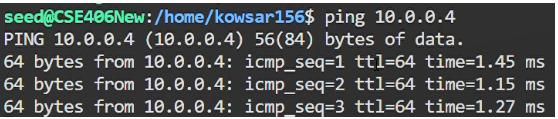
\includegraphics{images/ping}
        \end{figure}

        \item Now go to the terminal of the host machine (which is snort enabled) and see alerts
        \begin{figure}[h]
            \centering
            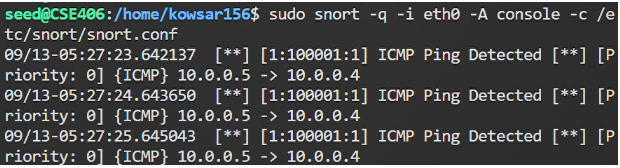
\includegraphics{images/sniff_alert}
        \end{figure}
    \end{itemize}

    \item \textbf{\large{Packet Logging (Logger Mode):}}
    \begin{itemize}
        \item From attacker machine:\\ 
        \textbf{ping 10.0.0.4}\\
        - This command sends ICMP packets to the host machine (10.0.0.4)
        \textbf{ftp 10.0.0.4}\\
        - This command tries to establish an FTP connection with the host machine (10.0.0.4)\\
        \begin{figure}[h]
            \centering
            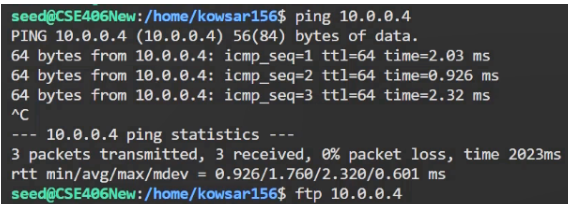
\includegraphics[width=0.8\textwidth]{images/ping_ftp}
        \end{figure}

        \item Now go to the terminal of the host machine (which is snort enabled) and see alerts\\
        \begin{figure}[h]
            \centering
            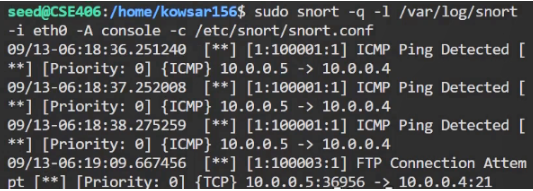
\includegraphics[width=0.8\textwidth]{images/log_alert_console}
        \end{figure}

        \item From host machine:\\
        \textbf{cd /var/log}
        - This command opens the directory where Snort is waiting with the log files\\
        \textbf{sudo chmod 777 snort}
        - This command gives necessary permissions to enter into the Snort folder\\
        \textbf{cd snort}
        - Through this command we enter the /var/log/snort directory where all the log files are kept\\
        \textbf{sudo chmod 777 snort.log.1694527894}
        - This command serves with necessary permissions to work on wireshark with the log file\\
        \begin{figure}[h]
            \centering
            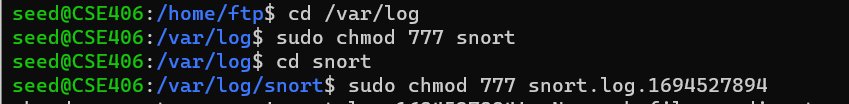
\includegraphics[width=0.8\textwidth]{images/cd}
        \end{figure}

        \item \textbf{vncserver -localhost no}\\
        - This allows the VM to be viewed by the Virtual Network viewer applications (e.g. TigerShark, RealVNC)\\
        \begin{figure}[h]
            \centering
            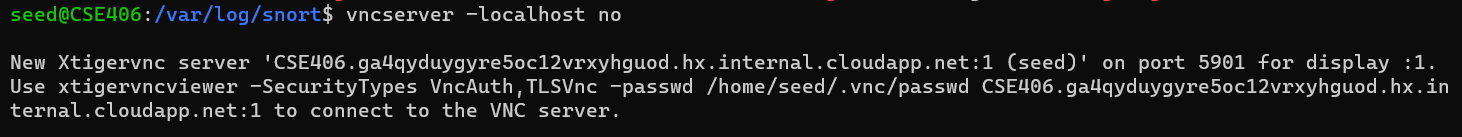
\includegraphics[width=0.95\textwidth]{images/vnc}
        \end{figure}

        \item Connect to your VM through TigerShark/RealVNC

        \item After entering the VM through TigerShark/RealVNC, \textbf{open WireShark → File → Open → /var/log/snort → snort.log.1694527894}\\
        \begin{figure}[h]
            \centering
            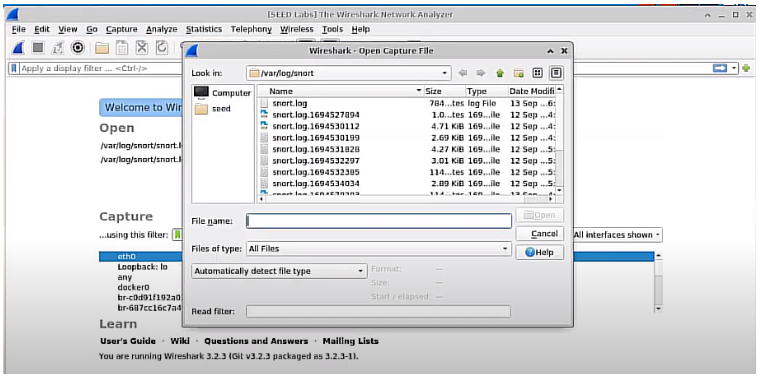
\includegraphics[width=0.8\textwidth]{images/open_file_wireshark}
        \end{figure}
        \begin{figure}[h]
            \centering
            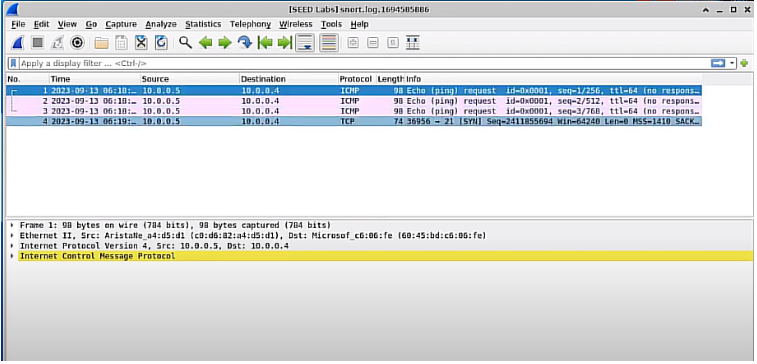
\includegraphics[width=0.8\textwidth]{images/examine_file_wireshark}
        \end{figure}
    \end{itemize}
\end{enumerate}
\vspace{0.4cm}

\section{Youtube Link}
https://www.youtube.com/watch?v=XaeAOnjMl-o

\end{document}
